\section{The impact of WF+DNS attacks}
\label{sec:analysis}
To evaluate out WF+DNS attacks we collected a dataset of traffic traces in May
2016 using TBB 5.5.4.
TBB was modified to not generate network traffic on launch (check for
updates, extensions etc) and
tor (bundled with TBB) to log incoming and outgoing cells together with
their size. We collected 100 samples of Alexa top 1k and one sample each of
Alexa top (1k,101k]. The order of site and sample collection was randomly
distributed to a Docker fleet, where each sample used a fresh circuit without
guards and a fresh copy of TBB\footnote{The consensus was cached to not
cause an excessive load on the network.} for up to 60 seconds,
in line with the recommendations by Wang and Goldberg~\cite{Wang2013a}.
We considered a sample collected if we managed to resolve the domain of the site
and did not prune our dataset further, neglecting issues like CloudFlare
CAPTCHAs, outliers and localized domains~\cite{Juarez2014a}. This may result
in worse results for all attacks~\cite{Wang2013a}, but we are primarily
interested in showing a difference between the WF attack and WF+DNS attacks.

We perform 10-fold cross-validation for all of our experiments in the open
world setting, monitoring 1000 sites with 100 instances each and
$100*1000$ unmonitored sites unless otherwise stated.
Note the 1:1 ratio between monitored traces and unmonitored traces,
ensuring that for the classifier there is equal probability in the testing
phase that a trace is a monitored or unmonitored site.
In other words, the \emph{base rate} is 0.5 in our experiments.
Furthermore, for all experiments we specify the starting Alexa rank of the
monitored sites
\emph{when simulating sites visited over the Tor network}\footnote{We always
use the same sample data for website fingerprinting.}.
Whem minitoring 1000 sites starting at rank 1, sites
[1,1000] are monitored and Alexa [1001,101000] unmonitored. Starting to
monitor Alexa from rank 100 means that Alexa sites [101,1100] are monitored,
and Alexa [1,100] and [1101,10100] unmonitored.
We never monitor an unmonitored site or vice versa.
How popular monitored sites
are is a key factor in the effectiveness of our attacks.
% note: base rate is per user, while popularity in Alexa for DNS observations
% is world-wide

Figure~\ref{fig:wfdns:torpct} shows the recall and precision for our WF+DNS
attacks as a function of the percentage of observed Tor exit bandwidth by the
attacker monitoring Alexa sites from rank $10^5$.
% TODO: consider moving recall and precision to background
Recall measures the probability that a visit to a monitored page will
be detected, while precision measures the probability that a classification by
the classifier of a visit to a monitored site (positive test outcome) is the
correct one. %Note that precision captures the base rate in an experiment.
For recall both \texttt{ctw} and \texttt{hp} are bound by the
percentage of exit bandwidth observed by the attacker (the percentage is an
upper bound).
Simply put, an attacker cannot identify a monitored site in the DNS data that
she does not see. Note that \texttt{ctw} sees improved recall over \texttt{wf}
at 100\% of exit bandwidth. For \texttt{hp} the results suggest that:

\begin{equation}
	\label{eq:hprecall}
	\textnormal{recall}_{\texttt{hp}} = \textnormal{recall}_{\texttt{wf}} * \textnormal{pct}
\end{equation}
Note that the above relationship only holds when observing DNS requests gives
a clear advantage to \texttt{hp} terms of precision over \texttt{wf} (see
following paragraph).
For precision our attacks have an imediate gain over \texttt{wf} as soon as
the attacker can observe \emph{any exit bandwidth}.
While the \texttt{hp} attack has constantly near-perfect precision, the
\texttt{ctw} attack benefits from observing more and more of exit bandwidth,
nearly reaching the same levels as \texttt{hp} at 100\%.


\begin{figure}[t]
\centering
\subfigure[Recall]{
	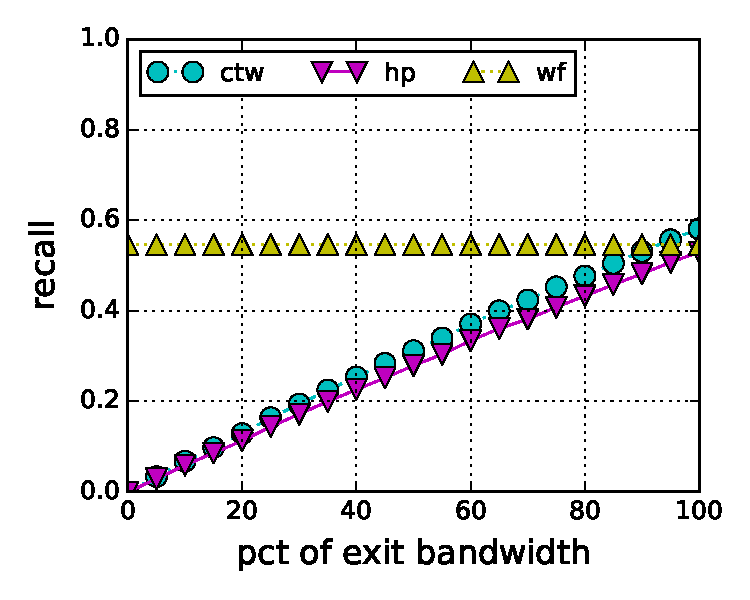
\includegraphics[width=0.466\linewidth]{figures/wfdns/pct/1kx100+100k-recall}
    \label{fig:wfdns:torpct:recall}
}
\subfigure[Precision]{
	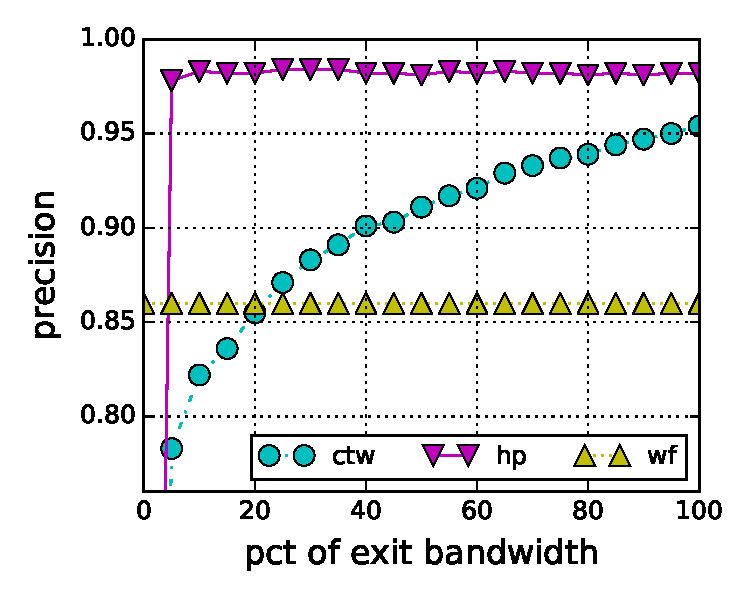
\includegraphics[width=0.466\linewidth]{figures/wfdns/pct/1kx100+100k-precision}
    \label{fig:wfdns:torpct:precision}
}
\caption{The recall and precision for an open-world dataset, monitoring sites
starting from Alexa rank 10k, comparing our attacks (\texttt{ctw and
 \texttt{hp}}) to a website fingerprinting attack (\texttt{wf}) for different
 percentages of observed exit bandwidth. }
\label{fig:wfdns:torpct}
\end{figure}


Figure~\ref{fig:wfdns:alexa} shows recall and precision at 100 percent of
observed Tor exit bandwidth as a function of the starting Alexa rank of
monitored sites (we still monitor 1000 sites).
For low Alexa ranks there is no difference between our attacks and the
\texttt{wf} attack. This is because, even with a window of only 60 seconds,
it is virtually guaranteed that someone browsed to any of the most popular
sites over Tor. At Alexa rank $10^3$ and onward we see a clear divergence from
the \texttt{wf} attack for both recall and precision:
\texttt{ctw} can improve the recall and precision, while
\texttt{hp} offers almost perfect precision already at Alexa $10^4$.

\begin{figure}[t]
\centering
\subfigure[Recall]{
	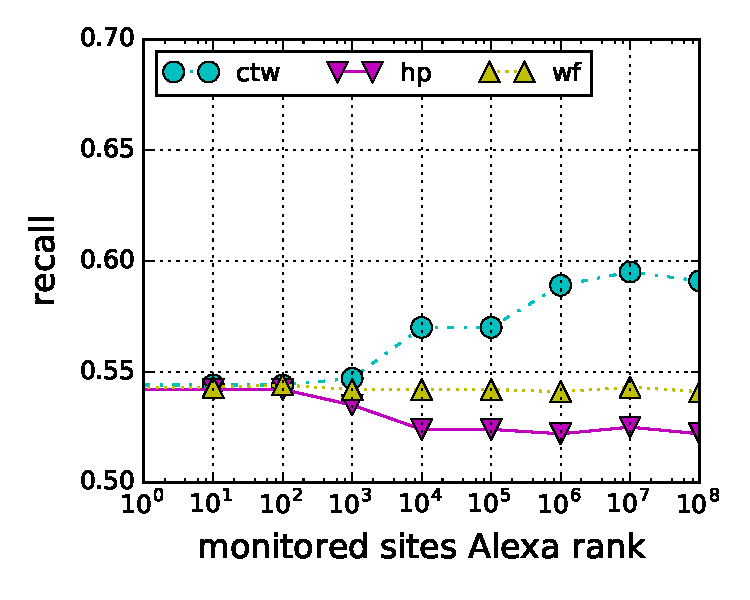
\includegraphics[width=0.466\linewidth]{figures/wfdns/alexa/1kx100+100k-offsets-100pct-recall}
    \label{fig:wfdns:alexa:recall}
}
\subfigure[Precision]{
	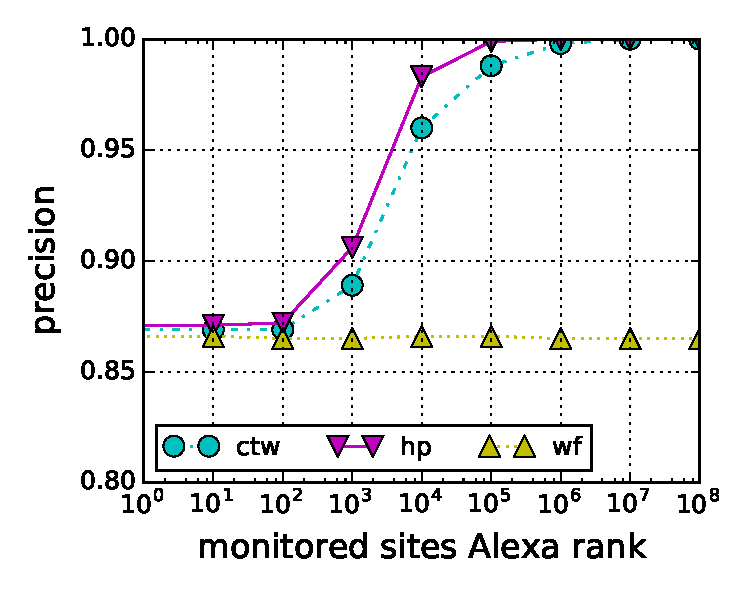
\includegraphics[width=0.466\linewidth]{figures/wfdns/alexa/1kx100+100k-offsets-100pct-precision}
    \label{fig:wfdns:alexa:precision}
}
\caption{The recall and precision when varying the starting Alexa rank of
monitored sites.}
\label{fig:wfdns:alexa}
\end{figure}

The above results paint a bleak picture: a small fraction of exit
bandwidth provides a perfectly precise attack on relatively
\emph{unpopular} sites such as \url{wikileaks.org} at Alexa rank 10808.
To better understand the implications and limitations of our attacks,
from now on we focus on
33\% of exit bandwith (as observed on average by Google) and
precision (where we see clear gain from both our attacks).
Unless otherwise stated
we monitor pages starting from Alexa $10^4$.

\begin{figure*}[t]
\centering
\subfigure[Approximating the impact of website fingerprinting defenses.]{
	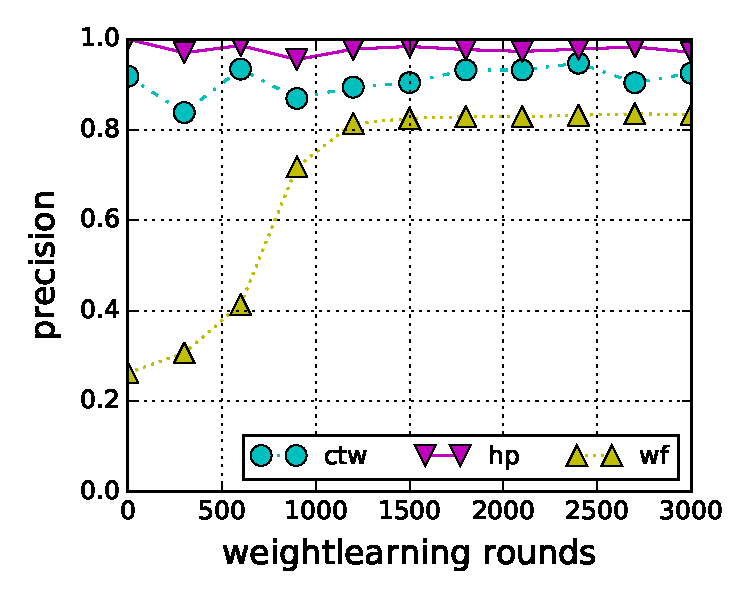
\includegraphics[width=0.23\linewidth]{figures/wfdns/rounds/100x100+10k}
    \label{fig:wfdns:var:rounds}
}
\subfigure[Increasing the window size due to TTL clipping at Alexa 10k and 100k.]{
	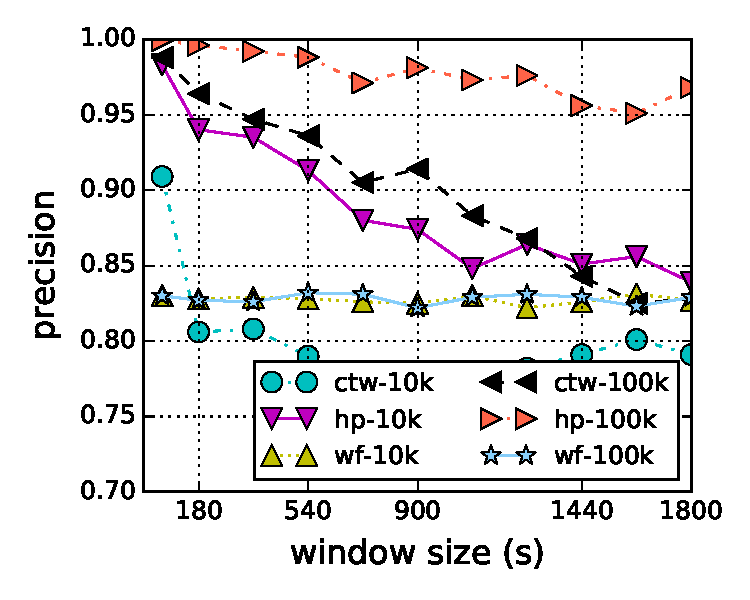
\includegraphics[width=0.23\linewidth]{figures/wfdns/window/100x100+10k}
    \label{fig:wfdns:var:window}
}
\subfigure[Scaling the Tor network wrt. site visits at Alexa 10k and 100k.]{
	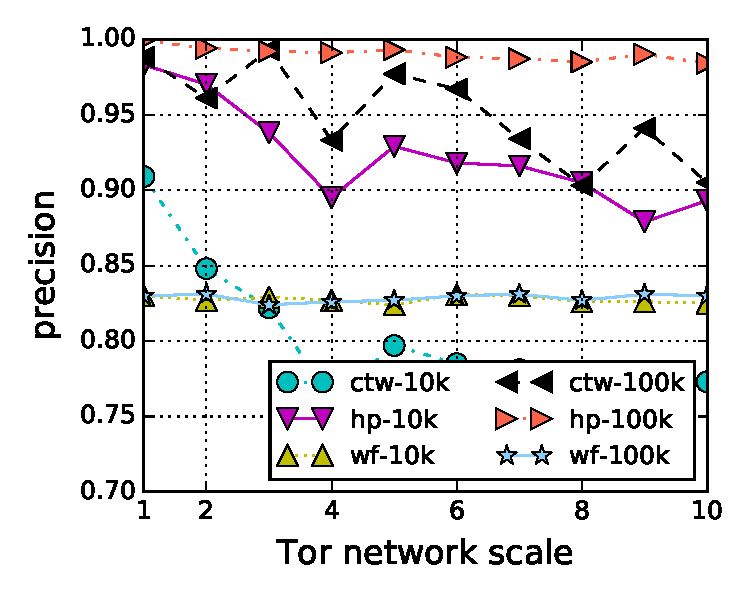
\includegraphics[width=0.23\linewidth]{figures/wfdns/scale/100x100+10k}
    \label{fig:wfdns:var:scale}
}
\subfigure[The impact of different website popularity distributions.]{
	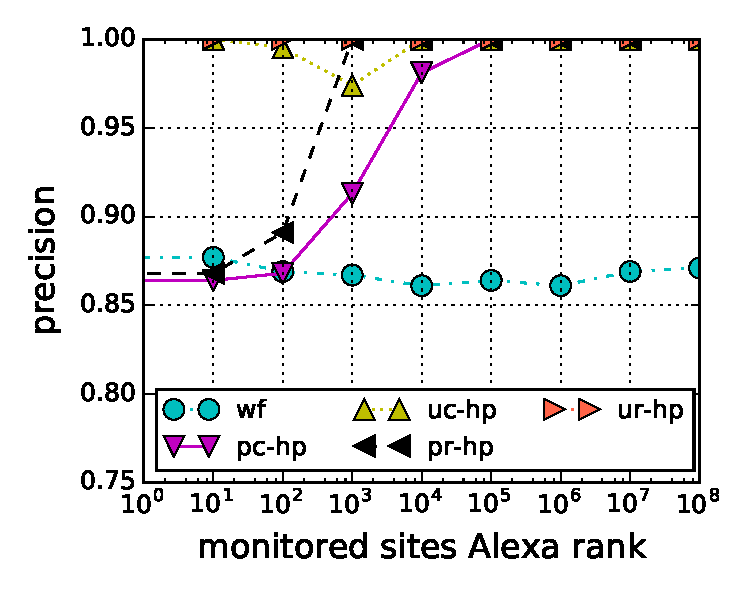
\includegraphics[width=0.23\linewidth]{figures/wfdns/dist/10x100+1k}
    \label{fig:wfdns:var:dist}
}
\caption{The impact on the precision of our attacks when observing 33\% of Tor
exit traffic (Google's average). The defaults are: 2500 weightlearning rounds,
60 seconds window size, Tor network scale 1.0, and the conservative
powerlaw distribution (pc) with $\alpha=1.13487087527372$.}
\label{fig:wfdns:var}
\end{figure*}

\subsection{Website fingerprinting defenses}
Website fingerprinting defenses are being
designed and discussed for deployment in Tor.
The defenses produce bandwidth and/or latency overhead with a significant
increase in overhead the stronger the defense\footnote{e.g., Juarez et al.
observe an exponentially growing bandwidth overhead for increasing protection
with WTF-PAD~\cite{DBLP:journals/corr/JuarezIPDW15}.}.
This leads to the goal of finding an optima with ``good enough''
protection and minimal overhead.
As a first attempt to approximate the impact of fingerprinting
defenses on WF+DNS attacks, we use Wa-kNN with
random weights and no weightlearning: this significantly reduces the
effectiveness of the attack since some features (like indices of outgoing
packers) are several orders of magnitude more useful
than others~\cite{DBLP:journals/corr/JuarezIPDW15}.
Figure~\ref{fig:wfdns:var:rounds} shows the impact of doing between 0 and 3000
rounds of weightlearning. At few to no rounds precision for the \texttt{wf}
attack is below 50\%---the classification is more likely to be wrong than
right---while there is no impact on the \texttt{hp} attack and a relatively
small decrease for the \texttt{ctw} attack.
For recall (not shown in the figure), note the bound and relationship in
\ref{eq:hprecall}: for \texttt{wf} at 0 rounds the recall is 0.055 and for
\texttt{hp} 0.019. This suggests that for WF defenses to
be effective against WF+DNS attacks the defense must be tuned to provide a
low recall even when the parameters of WF attacks are selected for high
recall.

\subsection{Tor's TTL clipping}
As noted in Section~\ref{sec:attack:sim}, due to a bug in Tor the max TTL
for DNS responses in an exit's cache is 60 seconds. As a consequence of this
a sliding window of only the last 60 seconds of all observed DNS requests is
enough to capture all visited monitored sites through Tor (subject to the
fraction of observed Tor exit bandwidth, and mapping DNS requests to sites).
Assume that the bug is fixed and the attacker keeps a window length equal
to the max TTL of all unique domains she found for her monitored sites.
Figure~\ref{fig:wfdns:var:window} shows the impact on precision for different
window sizes from 60 seconds to 30 minutes (Tor's MAX\_DNS\_ENTRY\_AGE
for keeping entries in an exit's cache) and for Alexa starting rank $10^4$ and
$10^5$. For \texttt{ctw}, the window size has a significant impact at both
Alexa starting ranks, while \texttt{hp} is only significantly impacted at
Alexa starting rank $10^4$: at higher ranks the DNS data still has a high
enough probability to give an advantage to the attacker despite the large
window size.

Recall that Table~\ref{tab:ttls} on page~\pageref{tab:ttls} shows statistics on
the minimum TTL of each site's unique domains. Our data shows that at least
half of the sites on Alexa top one million has a unique domain with a TTL of
60 seconds or below.
In fact, 48\% of the raw unique TTLs are below 60 seconds and only
26\% above 30 minutes. Fixing the Tor clipping bug is therefore not enough on
its own: to mitigate WF+DNS attacks the minimum TTL should be significantly
increased.

\subsection{A larger Tor network}
Figure~\ref{fig:wfdns:var:scale} scales the size of the Tor network wrt. site
visits from as-is to ten-times its size for Alexa starting rank $10^4$ and
$10^5$. At twice its current size, the impact on WF+DNS attacks is smaller than
increasing the minumum TTL for DNS caching to 180 seconds as shown in
Figure~\ref{fig:wfdns:var:window}. Clearly, WF+DNS attacks will not become
impractical for impopular sites as the network grows.

\subsection{Website popularity distributions}
% alexa offsets, all distributions and attacks
If we assume that our estimate for the number of sites visited through the Tor
network, as described in Section~\ref{sec:load-freq}, is roughly correct
(and we know from Figure~\ref{fig:wfdns:var:scale} that the impact of an error
is relatively minor) then one imporant consideration is how
these site visits are distributed. We define four distributions:
\begin{description}
	\item[pc] A conservative powerlaw distribution
	(with $\alpha=1.13487087527372$)
	that we manually fitted to the Alexa top 10k data,
	slightly underrepresenting the popularity of top Alexa sites.
	This distribution was described in Section~\ref{sec:attack:pop}.
	\item[pr] A realistic powerlaw distribution
	(with $\alpha=1.98331802607295$)
	that is the best fit according to
	the python powerlaw library by Alstott~et al.~\cite{powerlaw} for the Alexa
	top 10k data.
	\item[uc] A conservative uniformly random distribution that for some reason
	only considers one million active websites on the Internet.
	\item[ur] A realistic uniformly random distribution that considers 173 million active websites, as reported by Netcraft in July 2016.
\end{description}
Figure~\ref{fig:wfdns:var:dist} shows the impact on the precision of the
\texttt{hp} attack for the different distributions as we vary the starting
Alexa rank. The uniform distributions always have perfect precision.
The difference between the two powerlaw distributions is about one order of
magnitude in terms of starting Alexa rank: the realistic distribution gets
near perfect at $10^3$ and the conservative at $10^4$.
We conclude that WF+DNS attacks are perfectly precise for unpopular sites
where the probability that someone else than the target browses to a monitored
site within the timeframe given by the window length is negligible.

% limitation: webSITES, not wePAGES in our analysis + what we get from DNS.
